% template by Natalia Chernov for the University of Oldenburg

\documentclass[xcolor=table,9pt,aspectratio=169]{beamer}

\usepackage[utf8]{inputenc}

\usepackage{anyfontsize}
\usepackage[english,ngerman]{babel}
\usepackage{datetime}
\usepackage{helvet}
   \renewcommand{\familydefault}{\sfdefault}
\usepackage{lipsum}
\usepackage{lmodern}
\usepackage{multicol}
\usepackage{smartdiagram}
\usepackage{tikz}

\definecolor{uolblue}{RGB}{0,62,107}

\definecolor{blue1}{RGB}{0,78,159}
\definecolor{blue2}{RGB}{0,171,217}
\definecolor{blue3}{RGB}{91,197,242}
\definecolor{blue4}{RGB}{161,217,248}

\definecolor{green1}{RGB}{0,120,120}
\definecolor{green2}{RGB}{0,168,121}
\definecolor{green3}{RGB}{148,193,28}
\definecolor{green4}{RGB}{199,211,0}

\definecolor{orange1}{RGB}{213,59,10}
\definecolor{orange2}{RGB}{238,113,0}
\definecolor{orange3}{RGB}{243,145,0}
\definecolor{orange4}{RGB}{253,195,0}

\definecolor{gr}{RGB}{191,191,191}

\setbeameroption{hide notes}
% \setbeameroption{show only notes}
% \setbeameroption{show notes on second screen=right}

\setbeamertemplate{frametitle}{\color{uolblue}\fontsize{12}{20}\selectfont{\insertframetitle}}

\pgfdeclareimage[width=0.145\paperwidth]{logo}{figures/logo_uol_negative}
\pgfdeclareimage[width=0.072\paperwidth]{logo_small}{figures/logo_uol_negative}

\defbeamertemplate*{background canvas}{default_page}
{%
\begin{tikzpicture}
   \useasboundingbox (0,0) rectangle (\the\paperwidth,\the\paperheight);
   \filldraw[fill=uolblue,fill opacity=1,draw=none] (0,0) rectangle (0.119\paperwidth,\the\paperheight);
   \filldraw[fill=blue2,fill opacity=1,draw=none] (0.119\paperwidth,0) -- (0.119\paperwidth,0.565\paperheight) arc (117.2:180:0.6\paperwidth) -- cycle;
   \pgftext[at=\pgfpoint{10}{\the\paperheight-11.5},left,top]{\pgfsetfillopacity{1}\pgfuseimage{logo_small}};
\end{tikzpicture}
}
\defbeamertemplate*{background canvas}{titlepage_image}
{
\begin{tikzpicture}
   \useasboundingbox (0,0) rectangle (\the\paperwidth,\the\paperheight);
   \filldraw[fill=uolblue,fill opacity=1,draw=none] (0,0) rectangle (\the\paperwidth,\the\paperheight);
   \filldraw[fill=blue2,fill opacity=1,draw=none] (\the\paperwidth,0) -- (\the\paperwidth,0.66\paperheight) arc (90:180:0.6\paperwidth) -- cycle;
   \pgftext[at=\pgfpoint{14}{\the\paperheight-17.5},left,top]{\pgfsetfillopacity{1}\pgfuseimage{logo}};
\end{tikzpicture}
}
\BeforeBeginEnvironment{frame}{%
   \setbeamertemplate{background canvas}[default_page]%
}
\makeatletter
\define@key{beamerframe}{titlepage_image}[true]{%
   \setbeamercovered{invisible}%
   \setbeamertemplate{background canvas}[titlepage_image]%
}
\makeatother%

\setbeamertemplate{footline}
{
   \leavevmode
   \hbox{
   \hspace*{.025\paperwidth}\begin{beamercolorbox}[wd=.094\paperwidth,ht=2.25ex,dp=1ex,left]{}
   ~

   \vspace*{.042\paperheight}
      \fontsize{4.4}{5.9}\selectfont\color{white}\textbf{Slide \insertframenumber}\newline\insertdate
   \vspace*{.026\paperheight}
   \end{beamercolorbox}
   \hspace*{.05\paperwidth}\begin{beamercolorbox}
   [wd=.79\paperwidth,ht=2.25ex,dp=1ex,left]{}
   ~

   \vspace*{.042\paperheight}
      \fontsize{4.4}{5.9}\selectfont\color{black}\textbf{Poisoned Babies, Shot Fathers, and Ruined Experiments}\newline\color{gray}\insertauthor~--~University of Oldenburg, Faculty IV, Department of Philosophy
   \vspace*{.026\paperheight}
   \end{beamercolorbox}
   }
   \vskip0pt
}

\setbeamerfont{title}{size={\fontsize{22}{25}}}
\setbeamerfont{subtitle}{size={\fontsize{12}{14}}}
\setbeamerfont{author}{size={\fontsize{9}{11}}}
\setbeamerfont{date}{size={\fontsize{9}{11}}}
\setbeamercolor{title}{fg=white}
\setbeamercolor{subtitle}{fg=white}
\setbeamercolor{author}{fg=white}
\setbeamercolor{date}{fg=white}
\setbeamercolor{color_Logo-Platzhalter}{fg=white,bg=gray!40}

\defbeamertemplate*{title page}{customized}[1][]
{  \vspace*{20mm}
   \hspace*{-22.5mm}
   \begin{minipage}{\textwidth}
   \usebeamerfont{title}\usebeamercolor[fg]{title}\inserttitle\par
   \bigskip
   \usebeamerfont{subtitle}\usebeamercolor[fg]{subtitle}\insertsubtitle\par
   \bigskip
   \usebeamerfont{author}\usebeamercolor[fg]{author}\insertauthor,
   \usebeamerfont{date}\usebeamercolor[fg]{date}\insertdate\par
   \end{minipage}
}
\setbeamertemplate{navigation symbols}{}
\setbeamersize{text margin left=0.17\paperwidth,text margin right=0.04\paperwidth}

\title{Poisoned Babies, Shot Fathers,\\and Ruined Experiments}
\subtitle{Experimental Evidence in Favor of the\\Compositionality Constraint of\\Actual Causation}
\author{Alexander Max Bauer}
\date{16.09.2023}
\usepackage{enumitem}
\def\labelitemi{--}
\def\labelitemii{--}
\def\labelitemiii{--}

\begin{document}
{
\setbeamertemplate{footline}{}
\begin{frame}[titlepage_image]
   \maketitle
\end{frame}
}


%%%%%%%%%%%
% SLIDE 2 %
%%%%%%%%%%%
\begin{frame}{\vspace*{10mm}Roadmap}
\vspace*{-5mm}
\begin{itemize}
   \item[(1)] A Tale of Three Papers
   \item[(2)] Livengood and Sytsma (2020): ``Actual Causation and Compositionality''
   \item[(3)] Bauer and Romann (2022): ``Answers at Gunpoint''
   \item[(4)] Bauer and Kornmesser (2023): ``Poisoned Babies, Shot Fathers, and Ruined Experiments''
   \item[(5)] Takeaway Points
\end{itemize}
\end{frame}


%%%%%%%%%%%
% SLIDE 3 %
%%%%%%%%%%%
\begin{frame}{\vspace*{10mm}A Tale of Three Papers}
\vspace*{-5mm}
\begin{multicols}{3}
\begin{center}
   \frame{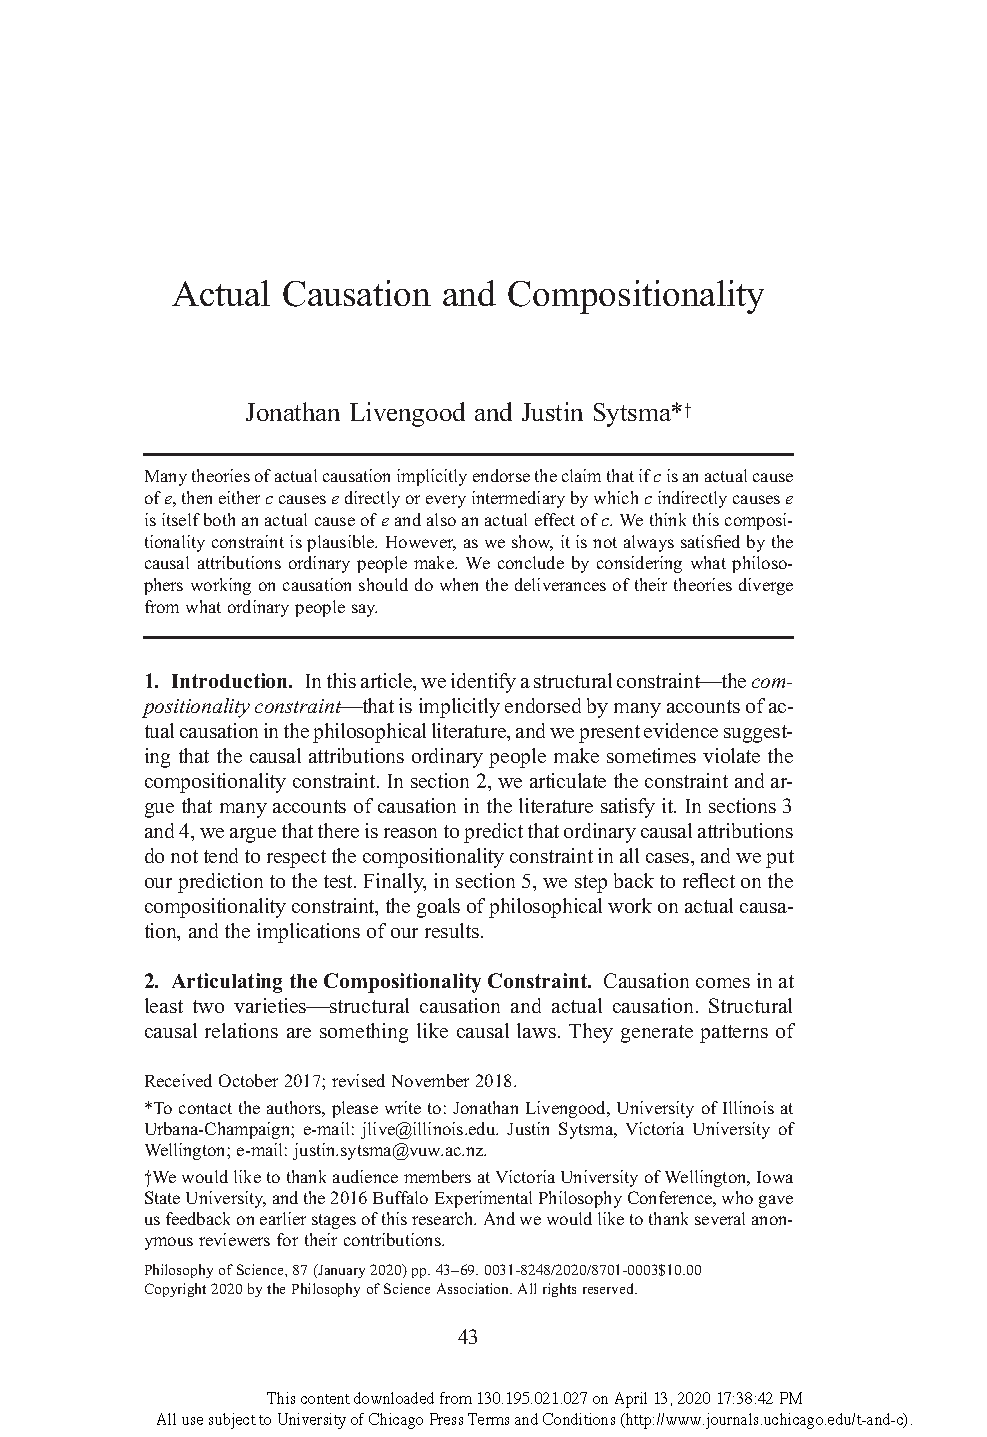
\includegraphics[width=\linewidth]{figures/livengood_sytsma_2020.pdf}}
   \frame{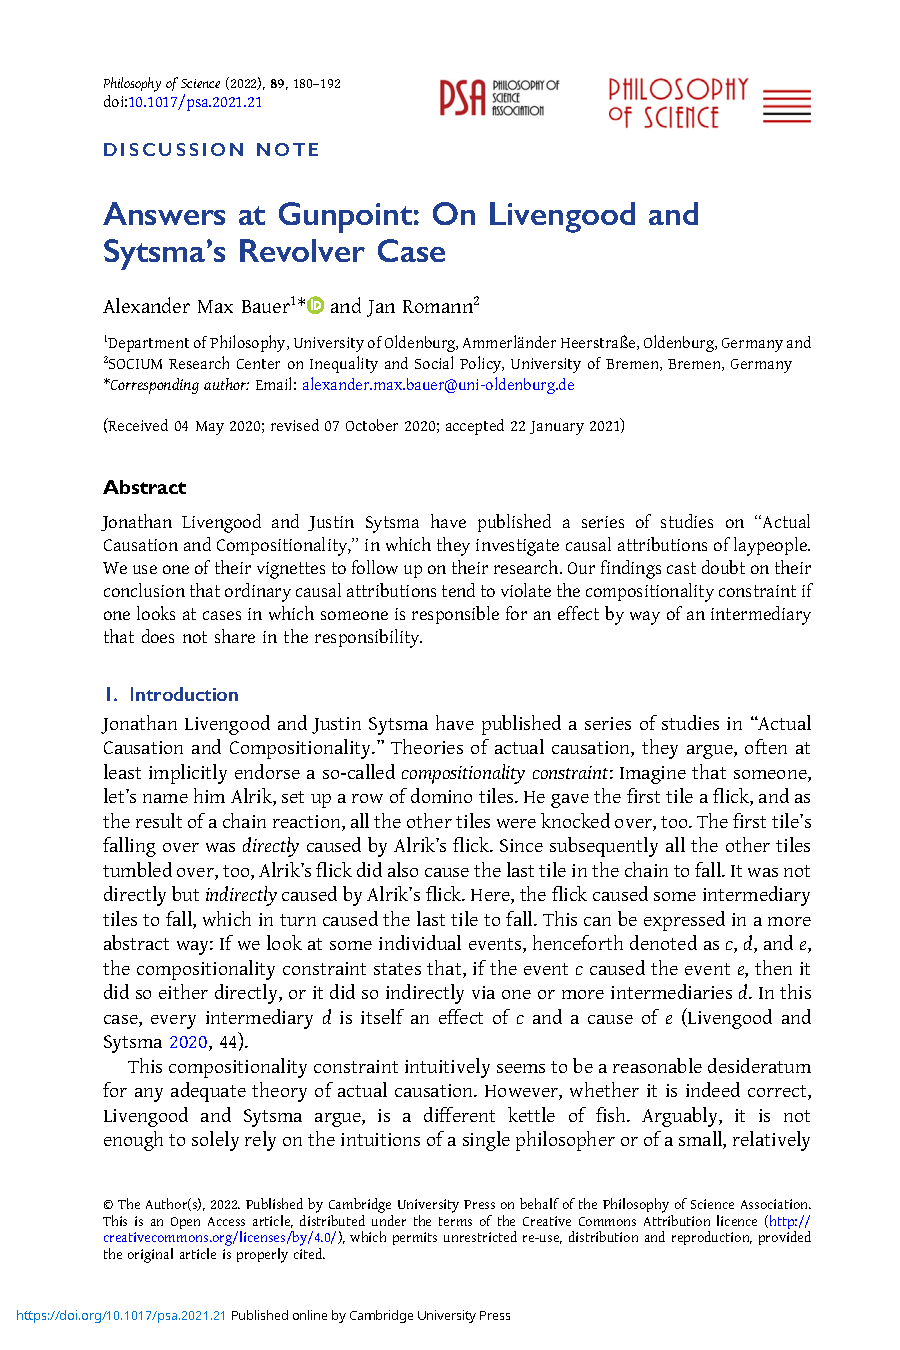
\includegraphics[width=\linewidth]{figures/bauer_romann_2022.pdf}}
   \frame{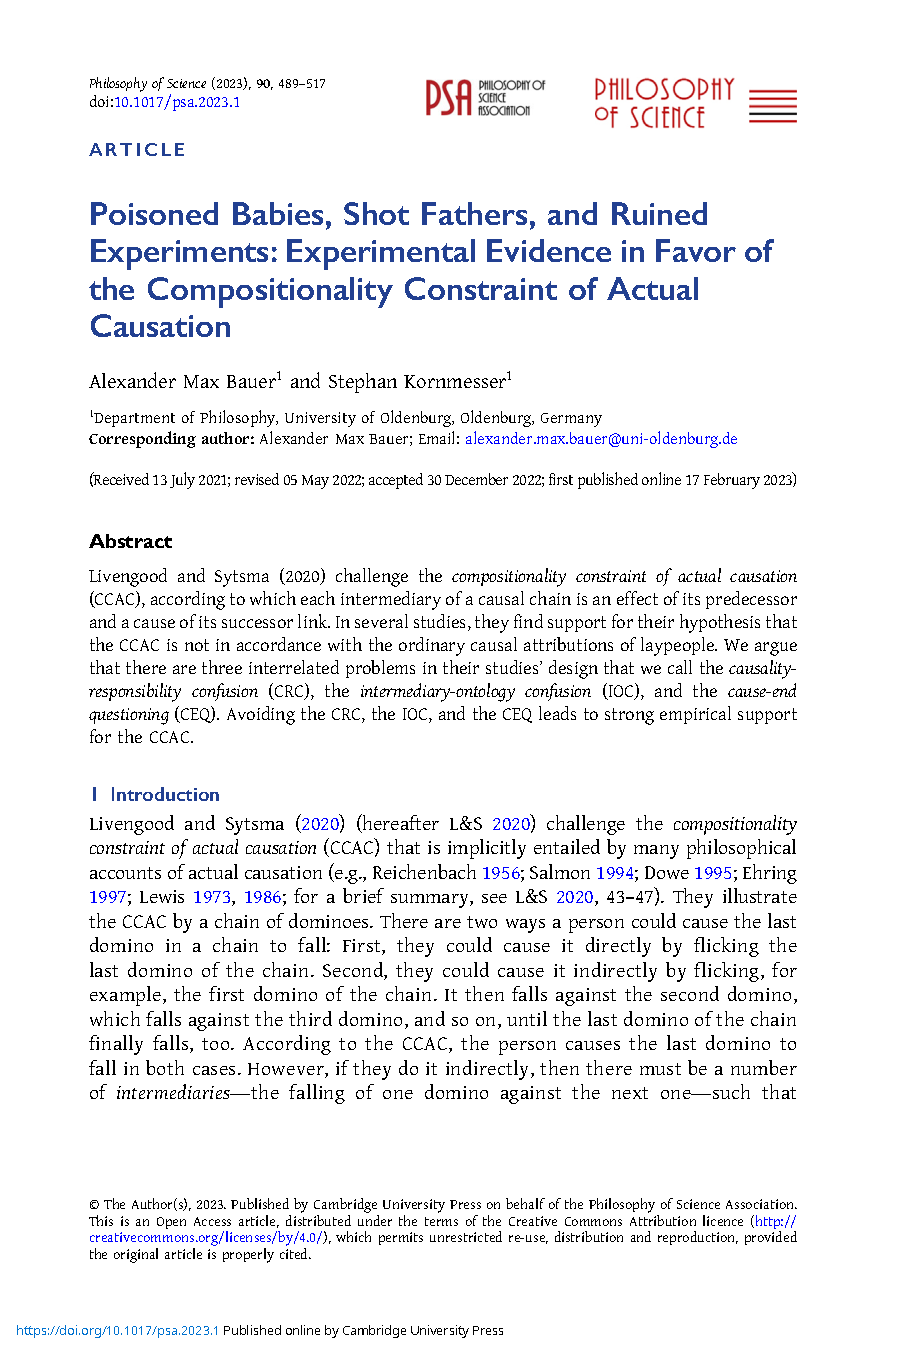
\includegraphics[width=\linewidth]{figures/bauer_kornmesser_2023.pdf}}
\end{center}
\end{multicols}
\end{frame}


%%%%%%%%%%%
% SLIDE 4 %
%%%%%%%%%%%
\begin{frame}{\vspace*{10mm}Livengood and Sytsma (2020): ``Actual Causation and Compositionality''}
\vspace*{-5mm}
\textbf{Compositionality Constraint of Actual Causation:} If $c$ is an actual cause of $e$, then either $c$ causes $e$ directly, or every intermediary $d$ by which $c$ indirectly causes $e$ is itself an actual effect of $c$ and an actual cause of $e$. \textcolor{gray}{(Livengood and Sytsma 2020, p. 44)}
\begin{center}
   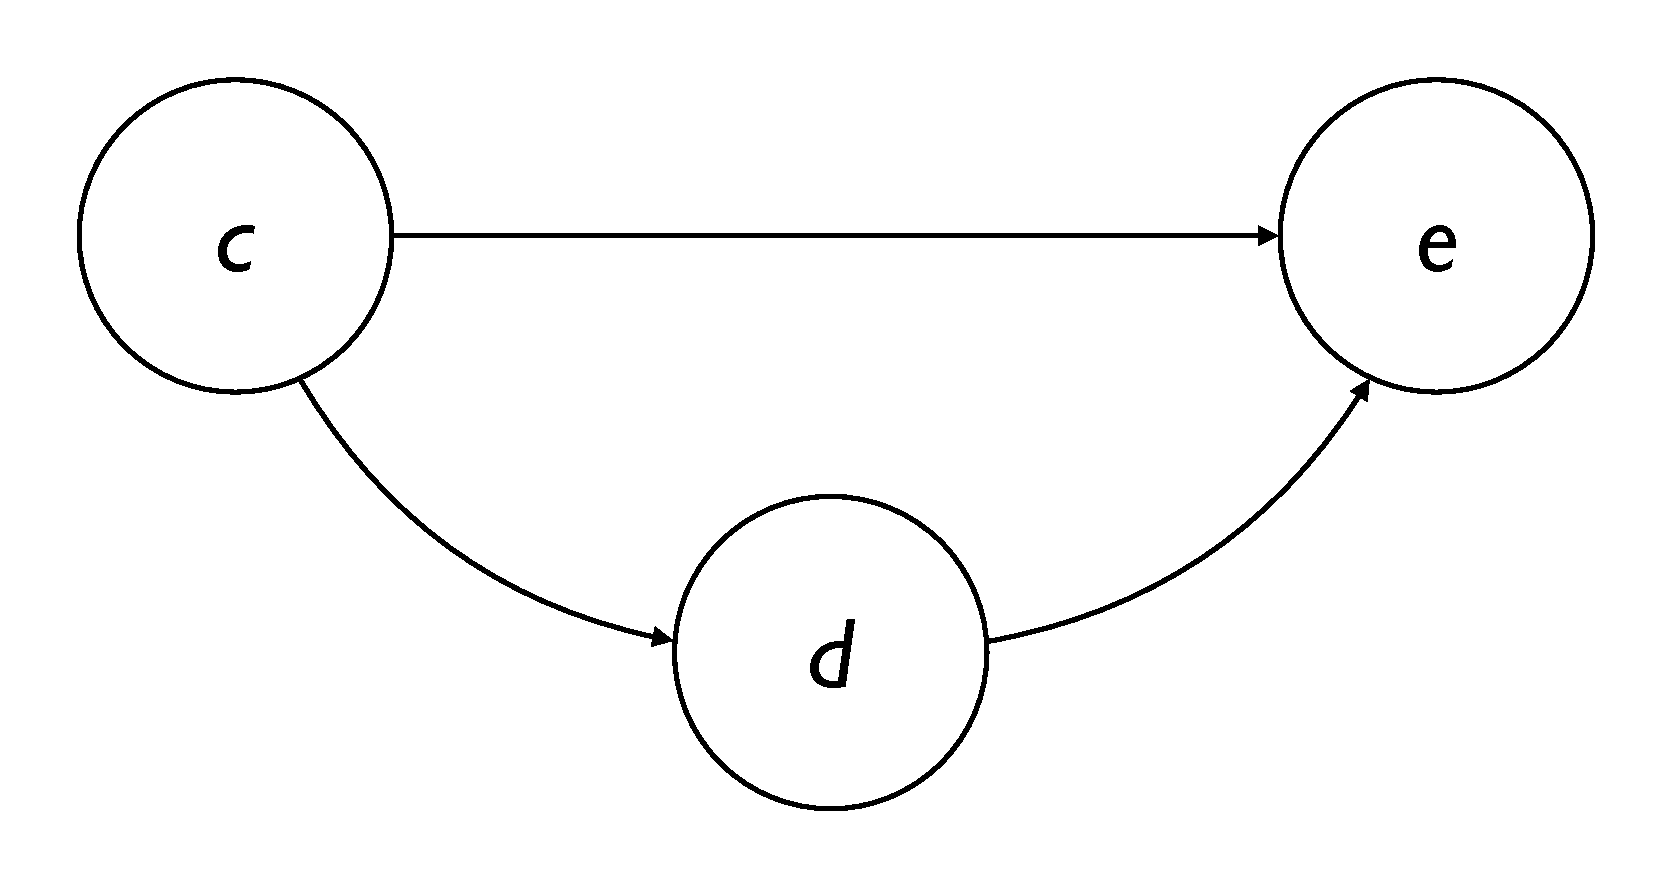
\includegraphics[width=0.5\linewidth]{figures/constraint.pdf}
\end{center}
\end{frame}


%%%%%%%%%%%
% SLIDE 5 %
%%%%%%%%%%%
\begin{frame}{\vspace*{10mm}Livengood and Sytsma (2020): ``Actual Causation and Compositionality''}
\vspace*{-5mm}
\textbf{Revolver Case:} Trent has decided to kill his father, Brad. He aims his loaded revolver at Brad and pulls the trigger, releasing the hammer. The hammer strikes the cartridge, igniting the gun powder. The gun powder explodes, driving the bullet from the gun. The bullet hits Brad in the head. He dies instantly. \textcolor{gray}{(Livengood and Sytsma 2020, p. 59)}
\begin{center}
   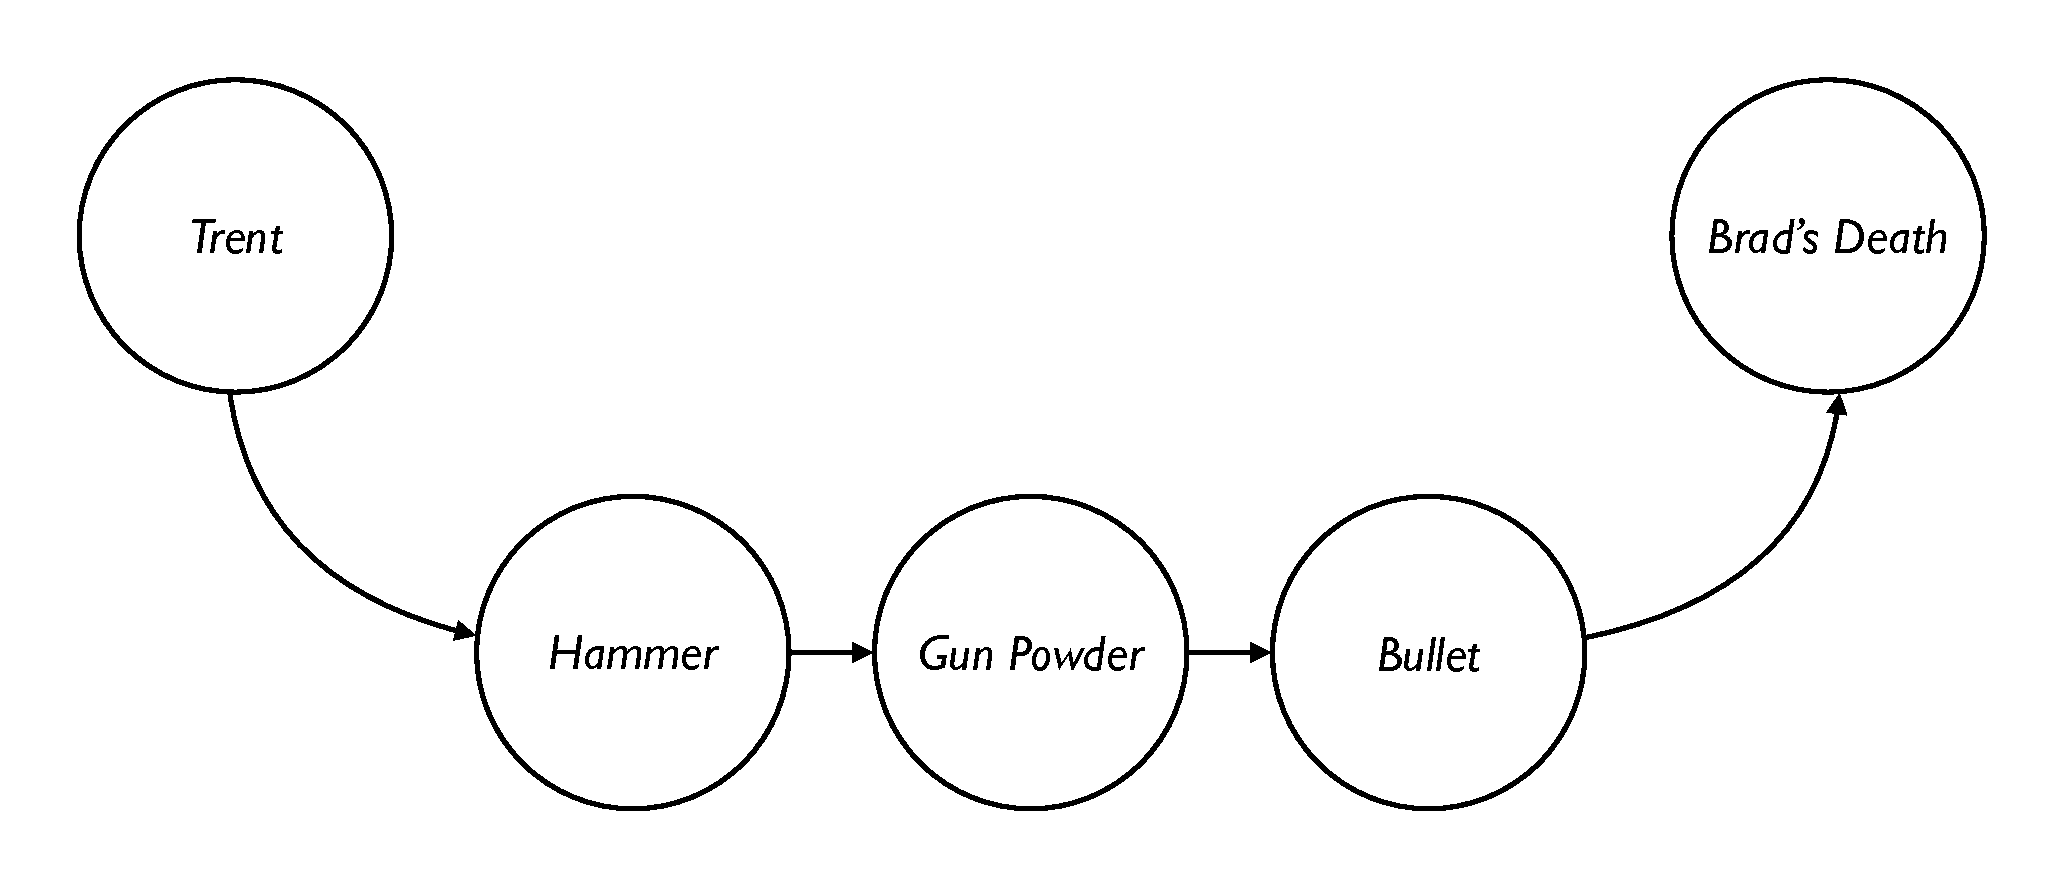
\includegraphics[width=0.75\linewidth]{figures/revolver.pdf}
\end{center}
\end{frame}


%%%%%%%%%%%
% SLIDE 6 %
%%%%%%%%%%%
\begin{frame}{\vspace*{10mm}Livengood and Sytsma (2020): ``Actual Causation and Compositionality''}
\vspace*{-5mm}
\begin{multicols}{2}
\textbf{Revolver Case}
\begin{itemize}
   \item $N=51$
   \item (dis)agreement on 7-point scale
   \item 4 statements
   \begin{itemize}
      \item[(A)] ``Trent caused Brad's death.''
      \item[(B)] ``The hammer caused Brad's death.''
      \item[(C)] ``The gun powder caused Brad's death.''
      \item[(D)] ``The bullet caused Brad's death.''
   \end{itemize}
\end{itemize}
\vfill
\begin{center}
   \frame{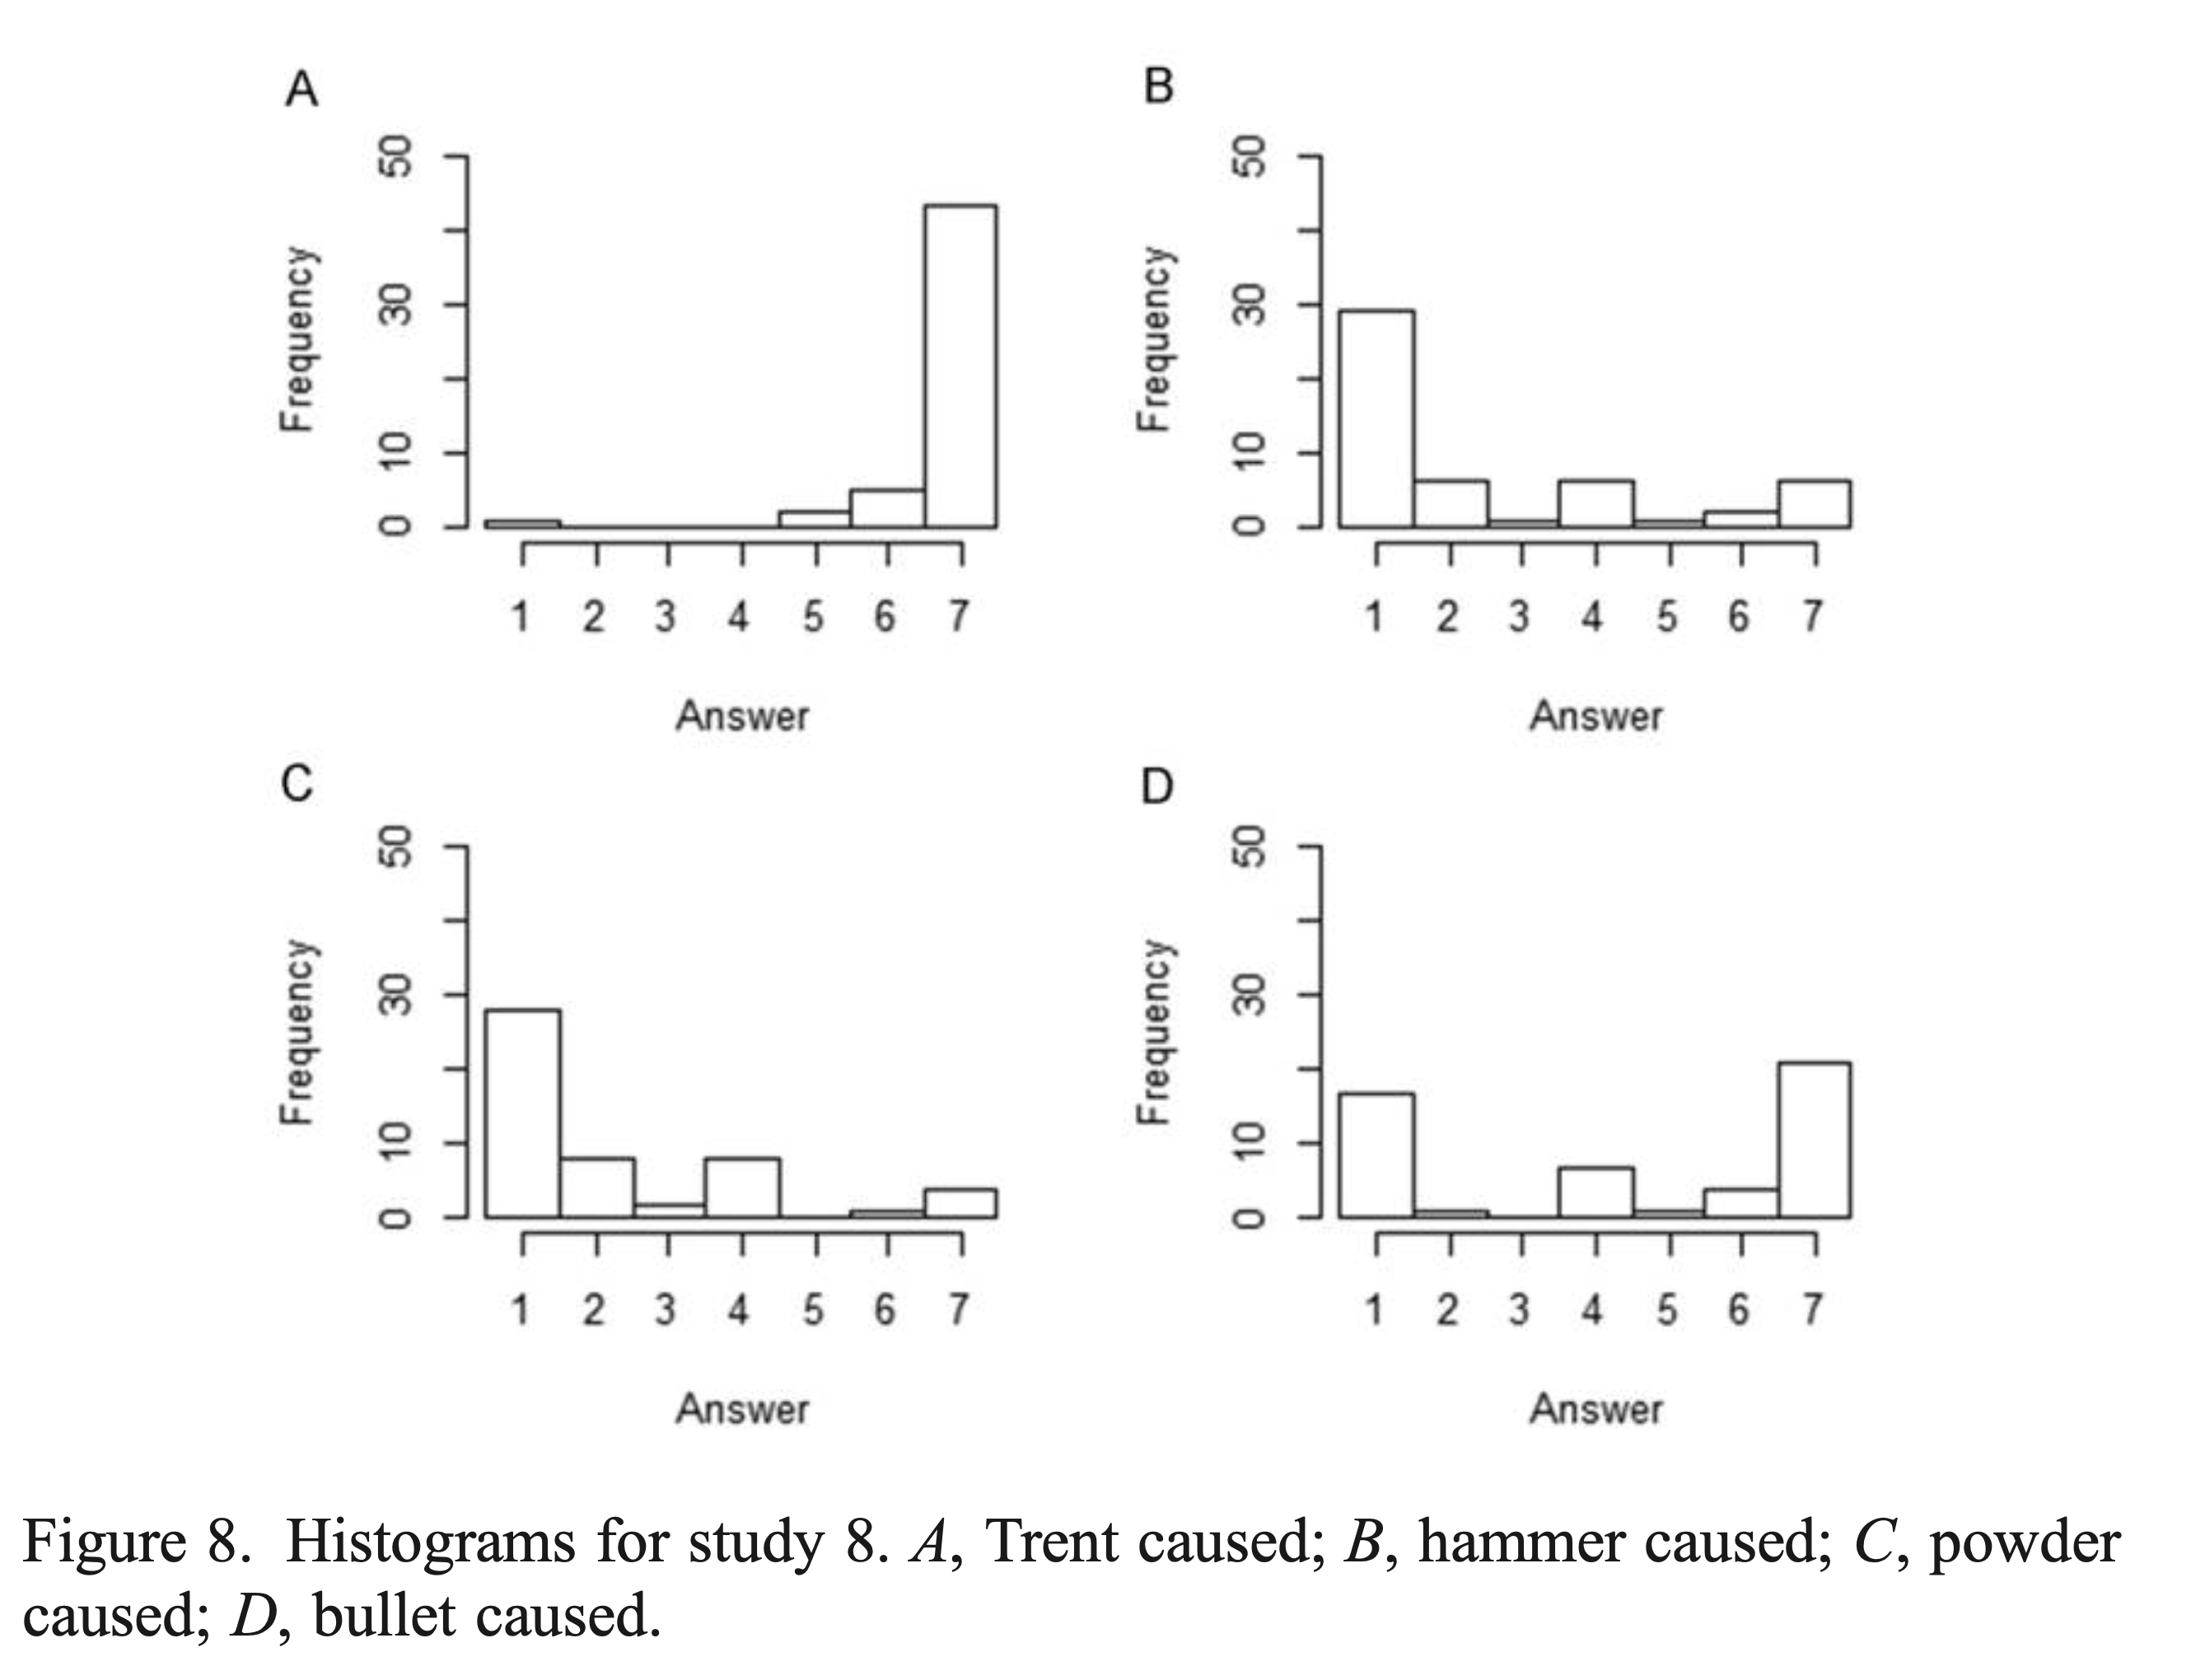
\includegraphics[width=\linewidth]{figures/livengood_sytsma_2020_fig_8.png}}
\end{center}
\end{multicols}
\end{frame}


%%%%%%%%%%%
% SLIDE 7 %
%%%%%%%%%%%
\begin{frame}{\vspace*{10mm}Bauer and Romann (2022): ``Answers at Gunpoint''}
\vspace*{-5mm}
\textbf{Events}\\
8 different events
\begin{itemize}
   \item[(A)] ``pulling the trigger''
   \item[(B)] ``releasing the hammer''
   \item[(C)] ``striking the cartridge''
   \item[(D)] ``igniting the gun powder''
   \item[(E)] ``the gun powder exploding''
   \item[(F)] ``driving the bullet from the gun''
   \item[(G)] ``the bullet hitting Brad in the head''
   \item[(H)] ``the death of Brad''
\end{itemize}
\vfill
\end{frame}


%%%%%%%%%%%
% SLIDE 8 %
%%%%%%%%%%%
\begin{frame}{\vspace*{10mm}Bauer and Romann (2022): ``Answers at Gunpoint''}
\vspace*{-5mm}
\textbf{Combinations of events}\\
28 ``X caused Y'' statements, e.\,g.,
\begin{itemize}
   \item[(A/B)] ``Pulling the trigger caused the release of the hammer.''
   \item[(C/D)] ``Striking the cartridge caused the ignition of the gun powder.''
   \item[(F/G)] ``The bullet being driven from the gun caused the bullet to hit Brad in the head.''
\end{itemize}
\hfill
\begin{center}
   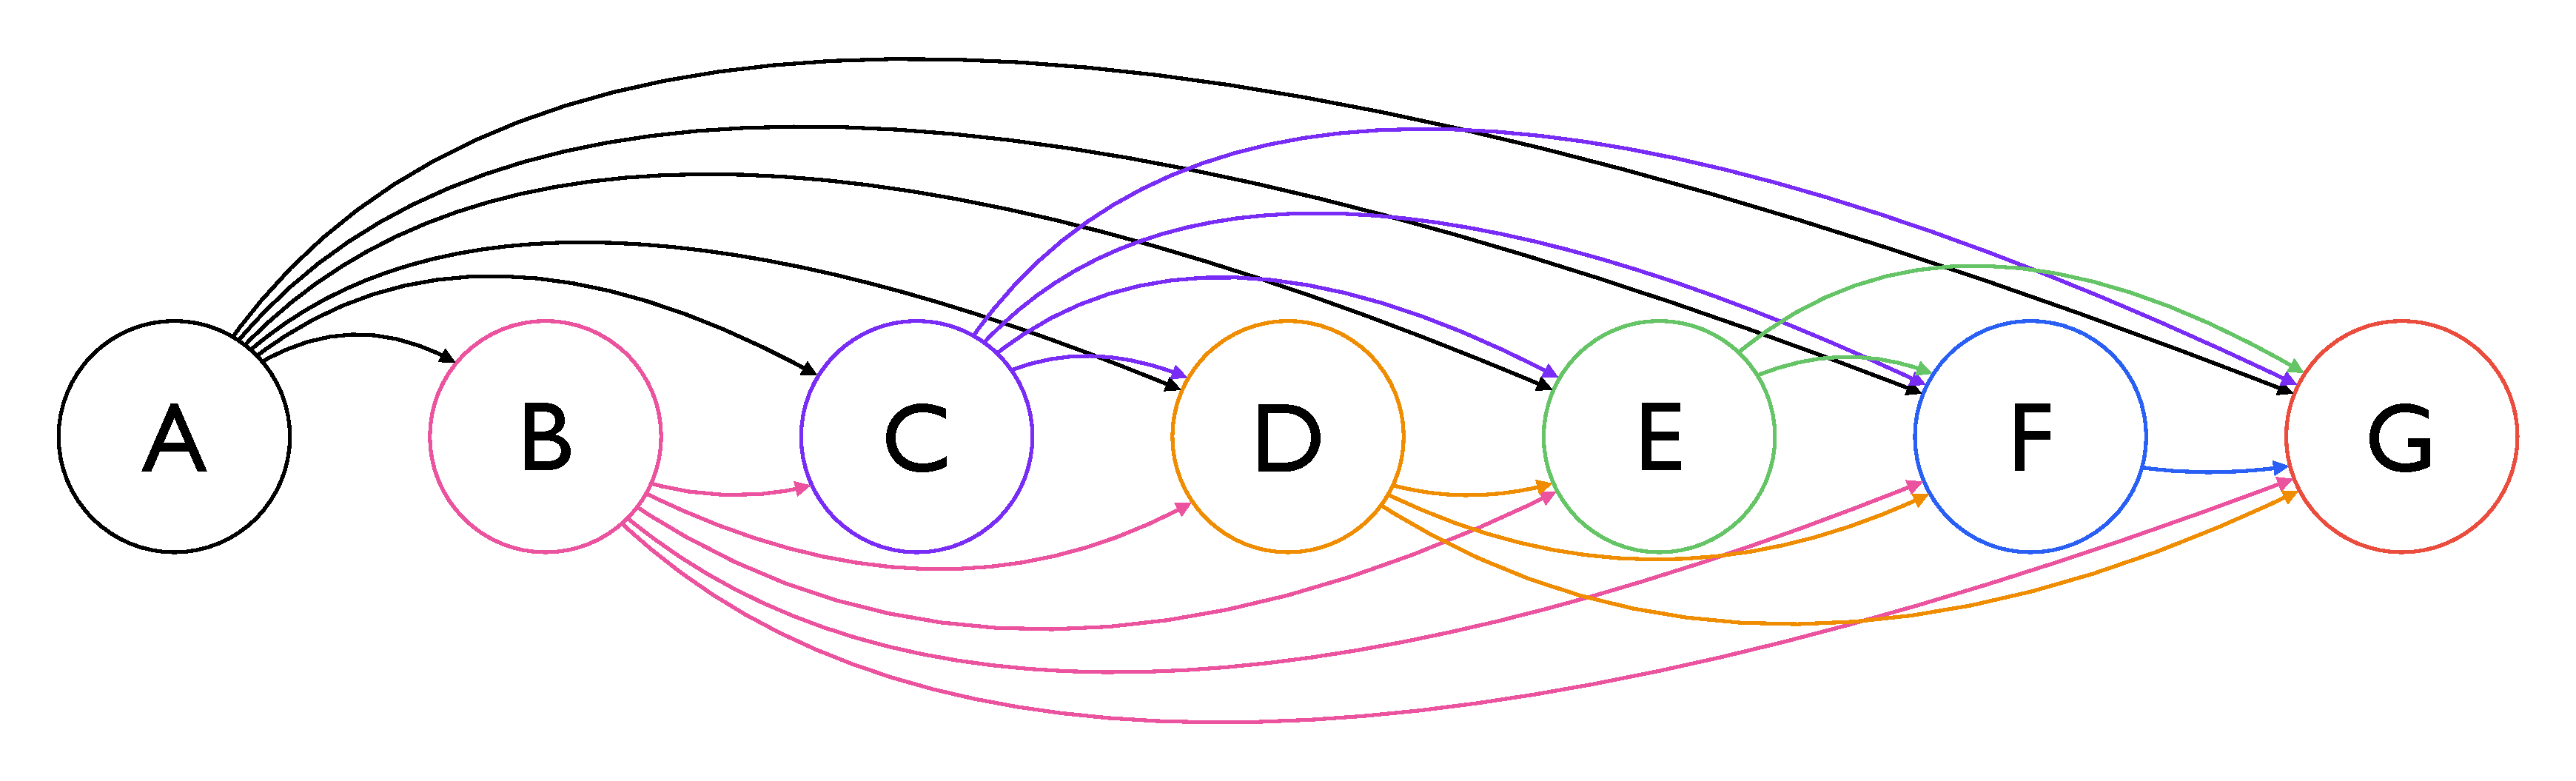
\includegraphics[width=.8\linewidth]{figures/combinations.pdf}
\end{center}
\end{frame}


%%%%%%%%%%%
% SLIDE 9 %
%%%%%%%%%%%
\begin{frame}{\vspace*{10mm}Bauer and Romann (2022): ``Answers at Gunpoint''}
\vspace*{-5mm}
\textbf{(More or less) Analogous Statements}\\
\begin{itemize}
   \item[(1)] ``Trent caused Brad's death.''
   \item[(A/H)] ``Pulling the trigger caused the death of Brad.''
\end{itemize}
\vspace*{0.5em}
\begin{itemize}
   \item[(2)] ``The hammer caused Brad's death.''
   \item[(B/H)] ``Releasing the hammer caused the death of Brad.''
\end{itemize}
\vspace*{0.5em}
\begin{itemize}
   \item[(3)] ``The gun powder caused Brad's death.''
   \item[(D/H)] ``Igniting the gun powder caused the death of Brad.''
   \item[(E/H)] ``The explosion of the gun powder caused the death of Brad.''
\end{itemize}
\vspace*{0.5em}
\begin{itemize}
   \item[(4)] ``The bullet powder caused Brad's death.''
   \item[(F/H)] ``The bullet being driven from the gun caused the death of Brad.''
   \item[(G/H)] ``The bullet hitting Brad in the head caused the death of Brad.''
\end{itemize}
\end{frame}


%%%%%%%%%%%%
% SLIDE 10 %
%%%%%%%%%%%%
\begin{frame}{\vspace*{10mm}Bauer and Romann (2022): ``Answers at Gunpoint''}
\vspace*{-5mm}
\begin{multicols}{2}
\textbf{Results}\\
\begin{itemize}
   \item $N=52$
   \item (dis)agreement on 7-point scale
   \item 28 statements
   \item central tendency for no statement smaller than the ``neutral'' value 4
\end{itemize}
\vfill
\begin{center}
   \frame{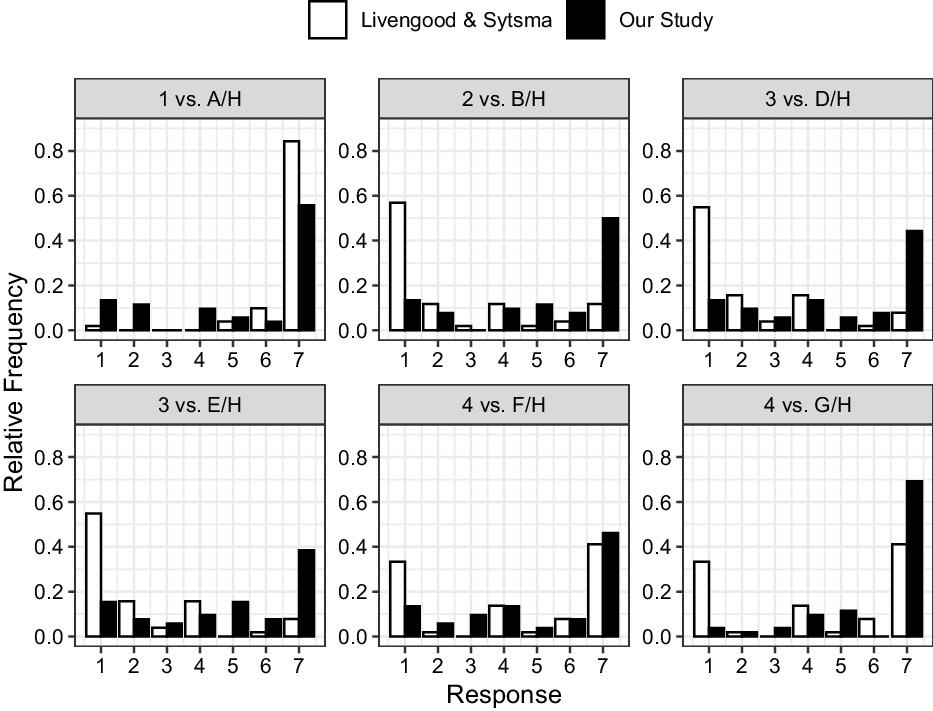
\includegraphics[width=\linewidth]{figures/bauer_romann_2020_fig_1.png}}
\end{center}
\end{multicols}
\end{frame}


%%%%%%%%%%%%
% SLIDE 11 %
%%%%%%%%%%%%
\begin{frame}{\vspace*{10mm}Bauer and Kornmesser (2023): ``Poisoned Babies, Shot Fathers, and Ruined Experiments''}
\vspace*{-5mm}
\textbf{Possible Explanations}\\
3 possible reasons for the difference
\begin{itemize}
   \item causality-responsibility confusion (CRC)
   \item intermediary-ontology confusion (IOC)
   \item cause-end questioning (CEQ)
\end{itemize}
\vfill
\end{frame}


%%%%%%%%%%%%
% SLIDE 12 %
%%%%%%%%%%%%
\begin{frame}{\vspace*{10mm}Bauer and Kornmesser (2023): ``Poisoned Babies, Shot Fathers, and Ruined Experiments''}
\vspace*{-5mm}
\textbf{Design}\\
\begin{itemize}
   \item vignettes from Livengood and Sytsma (2020)
      \begin{itemize}
         \item poisoned cup vignette
         \item revolver vignette
         \item GFCI vignette
      \end{itemize}
   \item studies for each vignette
      \begin{itemize}
         \item replication
         \item exclusion of IOC
         \item exclusion of CRC
         \item exclusion of CEQ
         \item simultaneous exclusion of IOC, CRC, and CEQ
      \end{itemize}
   \item $N\approx 60$ for each study (16 studies in total)
   \item (dis)agreement on 7-point scale
\end{itemize}
\vfill
\end{frame}


%%%%%%%%%%%%
% SLIDE 13 %
%%%%%%%%%%%%
\begin{frame}{\vspace*{10mm}Bauer and Kornmesser (2023): ``Poisoned Babies, Shot Fathers, and Ruined Experiments''}
\vspace*{-5mm}
\textbf{Results}\\
\begin{itemize}
   \item successful replication \textcolor{gray}{(for all vignettes)}
   \item excluding IOC led to less disagreement that intermediaries were causes \textcolor{gray}{(for poisoned cup and revolver vignette)}
   \item excluding CRC led to agreement that intermediaries were causes \textcolor{gray}{(for poisoned cup and revolver vignette)}
   \item excluding CEQ led to agreement that intermediaries were causes \textcolor{gray}{(for all vignettes)}
   \item simultaneous exclusion of IOC, CRC, and CEQ led to agreement that intermediaries were causes \textcolor{gray}{(for all vignettes)}
\end{itemize}
\vfill
\note{
   \begin{itemize}
      \item \textbf{IOC:} replacing individuals/objects with events reduces responsibility considerations/associations
      \item \textbf{CRC:} asking about the \textit{concept} of causation without using the ambiguous term ``to cause'' prevents from confusing causation with responsibility
      \begin{itemize}
         \item did not work for GFCI vignette, possibly due to preemption
      \end{itemize}
      \item \textbf{CEQ:} presenting a causal chain, where an intermediary $d_1$ is presented as a cause of a further intermediary $d_2$ instead of the chain's final element $e$, directs the focus to the \textit{concept} of causation; similar to Bauer and Romann (2022)
   \end{itemize}
}
\end{frame}


%%%%%%%%%%%%
% SLIDE 14 %
%%%%%%%%%%%%
\begin{frame}{\vspace*{10mm}Takeaway Points}
\vspace*{-5mm}
\textbf{Key Assumptions in Light of the Data}
\begin{itemize}
   \item if asked the right way, subjects can be prevented from confusing causation with responsibility
   \item subjects' intuitions are not in conflict with the Compositionality Constraint of Actual Causation \textcolor{gray}{(contrary to Livengood and Sytsma 2020)}
   \item responsibility might not be part of the concept of causation \textcolor{gray}{(contrary to proponents of the \textit{responsibility view})}
\end{itemize}
\vfill
\end{frame}


%%%%%%%%%%%%
% SLIDE 15 %
%%%%%%%%%%%%
\begin{frame}{}
\vspace*{-5mm}
\begin{center}
   {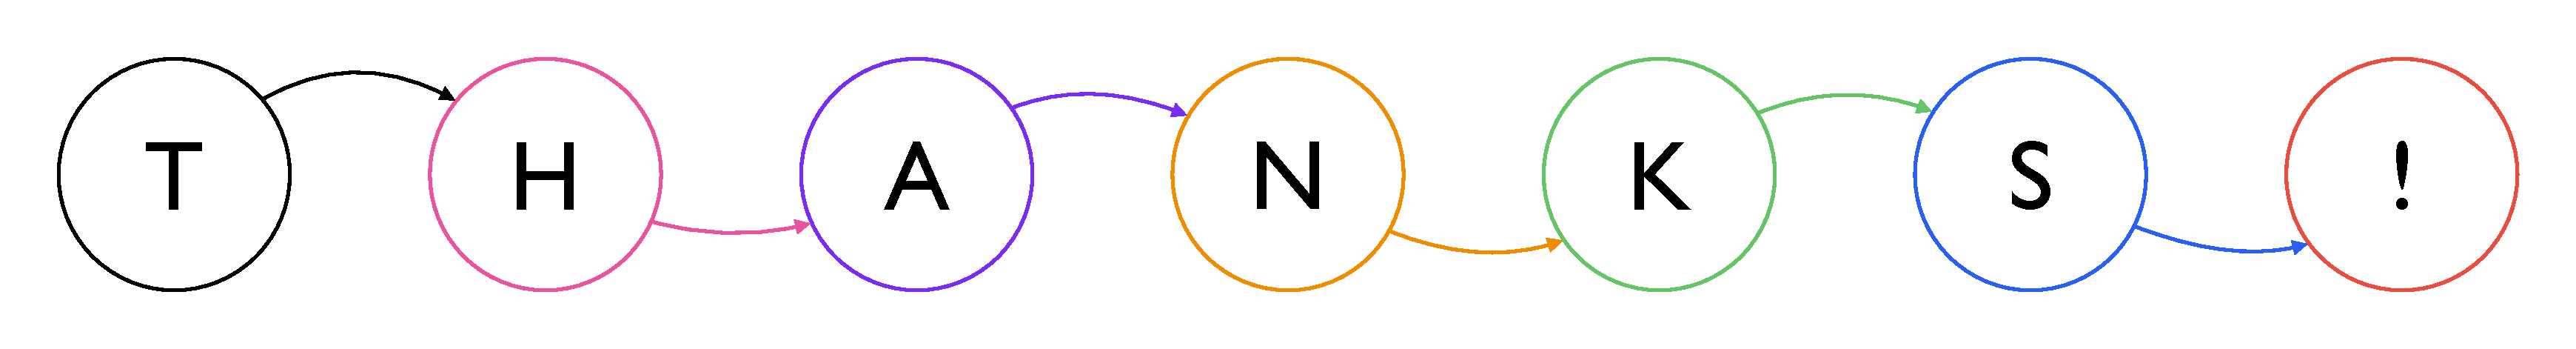
\includegraphics[width=\linewidth]{figures/thanks.pdf}}
\end{center}
\end{frame}


%%%%%%%%%%%%
% SLIDE 16 %
%%%%%%%%%%%%
\begin{frame}{\vspace*{10mm}Livengood and Sytsma (2020): ``Actual Causation and Compositionality''}
\vspace*{-5mm}
\textbf{Poisoned Cup Vignette:} Amy wants to kill her daughter, Jessica, but she doesn't want to go to prison for murder. As such, Amy hatches a plan. She arranges for a babysitter, Courtney, to take care of Jessica while she is out of town on business. Before leaving, Amy laces one of Jessica's sippy cups with a deadly poison that is very difficult to detect. That evening, Courtney gives Jessica juice in the poisoned sippy cup. Jessica drinks the juice and dies two hours later. \textcolor{gray}{(Livengood and Sytsma 2020, p. 49)}
\end{frame}


%%%%%%%%%%%%
% SLIDE 17 %
%%%%%%%%%%%%
\begin{frame}{\vspace*{10mm}Livengood and Sytsma (2020): ``Actual Causation and Compositionality''}
\vspace*{-5mm}
\textbf{GFCI Vignette:} John is a scientist conducting a very important experiment on an unusual species of plant. His experiment requires growing his plants under a special light, which is plugged into an outlet with a ground fault circuit interrupter (GFCI) safety mechanism. The pipes running to John's laboratory were correctly manufactured and installed, and the system was protected from any changes in weather condition.\par
\hspace{2em}Despite there being nothing wrong with the pipes, one day a pipe burst in John's laboratory. Water ran into the outlet powering the special light. A properly functioning GFCI safety mechanism will break the circuit so that no power flows through its outlet if exposed to water in this way. And in fact, the GFCI safety mechanism did break the circuit. The special light turned off and the experiment was ruined. \textcolor{gray}{(Livengood and Sytsma 2020, p. 62)}
\end{frame}


%%%%%%%%%%%%
% SLIDE 18 %
%%%%%%%%%%%%
\begin{frame}{\vspace*{10mm}Bauer and Romann (2022): ``Answers at Gunpoint''}
\vspace*{-5mm}
\begin{multicols}{2}
\begin{center}
   \frame{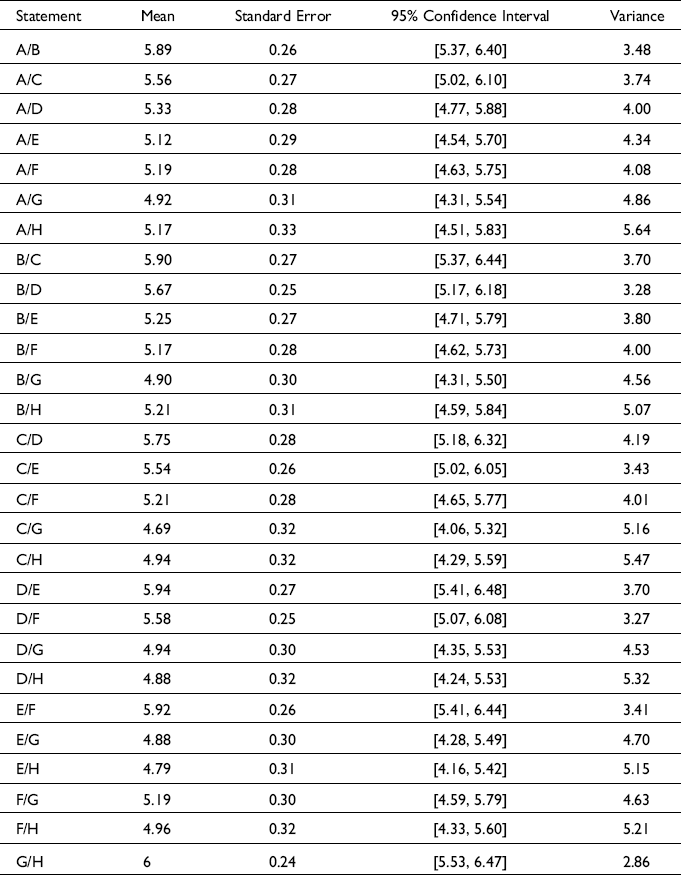
\includegraphics[width=0.5\linewidth]{figures/bauer_romann_2020_tab_1.png}}\\
   {\footnotesize\textbf{Table 1:} Summary of statements}\\
   \frame{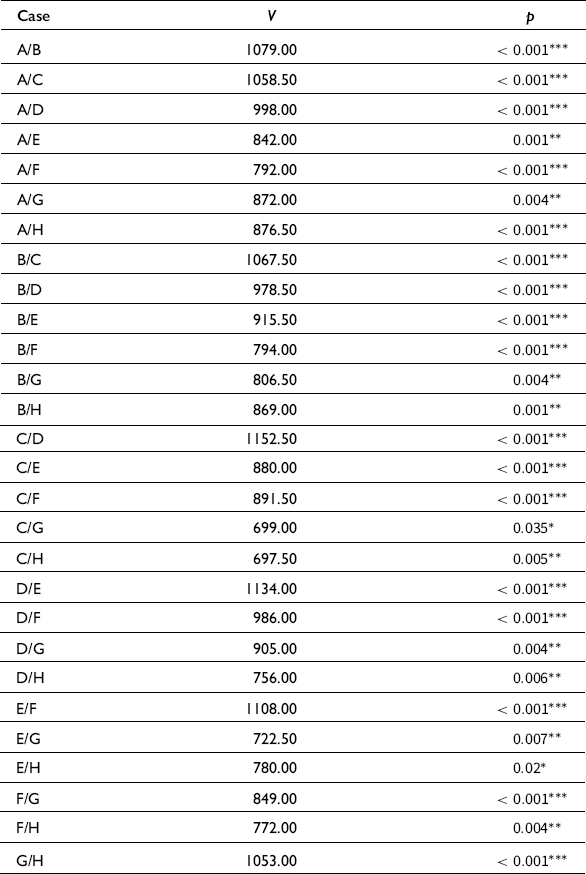
\includegraphics[width=0.5\linewidth]{figures/bauer_romann_2020_tab_2.png}}\\
   {\footnotesize\textbf{Table 2:} Two-tailed Wilcoxon signed-rank tests}
\end{center}
\end{multicols}
\end{frame}


%%%%%%%%%%%%
% SLIDE 19 %
%%%%%%%%%%%%
\begin{frame}{\vspace*{10mm}Bauer and Kornmesser (2023): ``Poisoned Babies, Shot Fathers, and Ruined Experiments''}
\vspace*{-5mm}
\begin{center}
   \frame{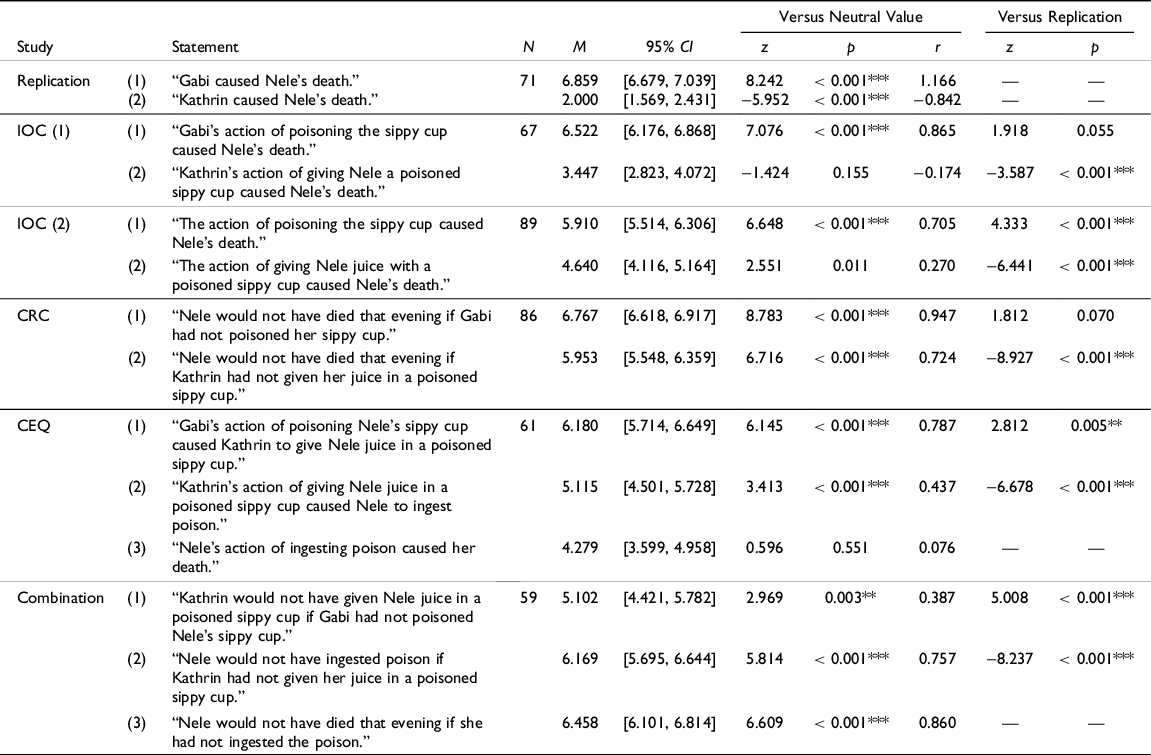
\includegraphics[width=0.5\linewidth]{figures/bauer_kornmesser_2023_tab_1}}\\
   {\footnotesize\textbf{Table 1:} Summary of statements for the poisoned cup vignette,\\reporting results of Wilcoxon signed-rank tests}
\end{center}
\end{frame}


%%%%%%%%%%%%
% SLIDE 20 %
%%%%%%%%%%%%
\begin{frame}{\vspace*{10mm}Bauer and Kornmesser (2023): ``Poisoned Babies, Shot Fathers, and Ruined Experiments''}
\vspace*{-5mm}
\begin{center}
   \frame{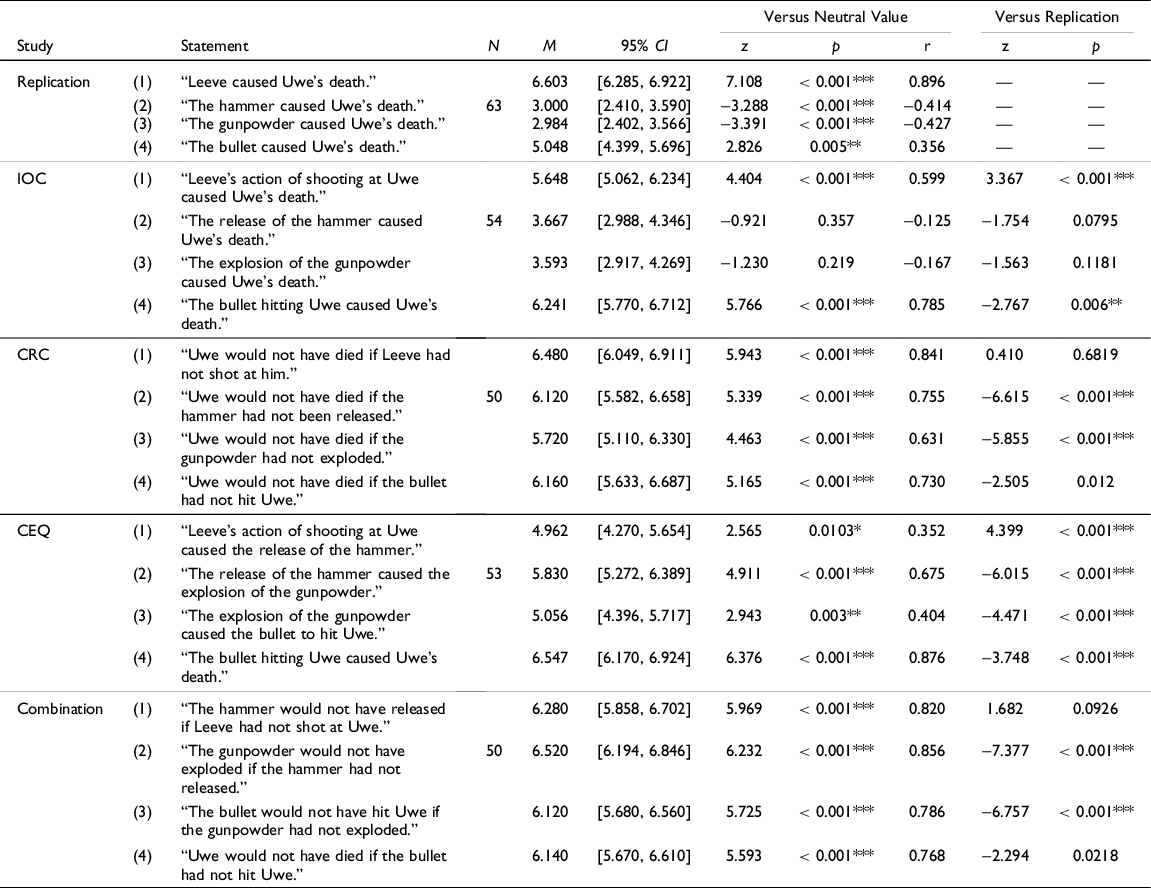
\includegraphics[width=0.5\linewidth]{figures/bauer_kornmesser_2023_tab_2}}\\
   {\footnotesize\textbf{Table 2:} Summary of statements for the revolver vignette,\\reporting results of Wilcoxon signed-rank tests}
\end{center}
\end{frame}


%%%%%%%%%%%%
% SLIDE 21 %
%%%%%%%%%%%%
\begin{frame}{\vspace*{10mm}Bauer and Kornmesser (2023): ``Poisoned Babies, Shot Fathers, and Ruined Experiments''}
\vspace*{-5mm}
\begin{center}
   \frame{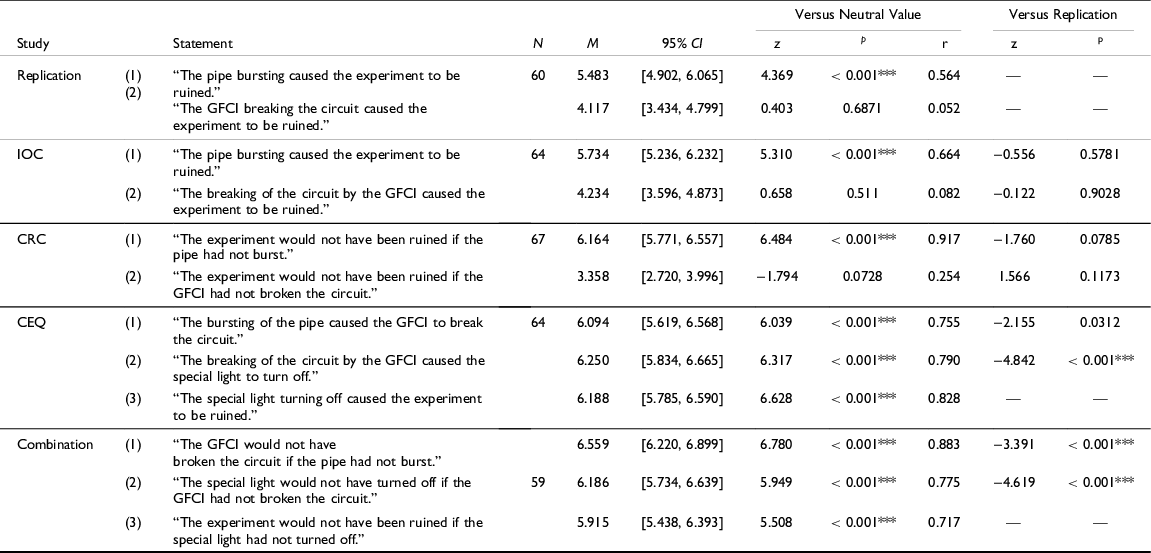
\includegraphics[width=0.5\linewidth]{figures/bauer_kornmesser_2023_tab_3}}\\
   {\footnotesize\textbf{Table 3:} Summary of statements for the GFCI vignette,\\reporting results of Wilcoxon signed-rank tests}
\end{center}
\end{frame}


\end{document}
